\section{Auswertung}
\label{sec:Auswertung}
Die Messung lief für eine Zeit von $t_{\text{Messung}} = \SI{250093}{\second} ≈ \SI{69.47}{\hour}$.
Während dieser Messzeit $t_{\text{Messung}}$ wurden $N_{\text{Start}} = \num{4185569}$ Startsignale und $N_{\text{Stop}} = \num{12355}$ Stoppsignale detektiert.
Der MCA hat insgesamt \num{10114} Ereignisse aufgenommen und auf $N_{\text{Kanal}} = \num{451}$ Kanäle gebinnt.
Die Suchzeit für den Versuch beträgt $T_{\text{Such}} = \SI{20}{\micro\second}$.
Damit ergibt sich eine Ereignissrate von:
\begin{equation*}
    \nu = \frac{N_{\text{Start}}}{t_{\text{Messung}}} = \SI{16.74 \pm 0.008}{\hertz}
\end{equation*}

\subsection{Untergrundrate}
Um zu berechnen wie groß die Untergrundrate ist, wird zunächst bestimmt welchen Anteil Myonen, die während einer laufenden Messung in den Tank fallen, vom Untergrund einnehmen.
Die Wahrscheinlichkeit $k$ weitere  Myonen in der Suchzeit $T_{\text{Such}}$ zu detektieren ist poissonverteilt und ergibt sich zu:
\begin{equation*}
    P_{T_{\text{Such}}\cdot \nu}(k) = \frac{(T_{\text{Such}}\cdot \nu)^k}{k!} e^{-(T_{\text{Such}}\cdot \nu)}
\end{equation*}
Damit ergibt sich die Wahrscheinlichkeit ein zusätzliches Myon zu messen zu: 
\begin{equation*}
    P_{T_{\text{Such}}\cdot \nu}(1) = (T_{\text{Such}}\cdot \nu)e^{-(T_{\text{Such}}\cdot \nu)} ≈ \SI{0.033460 \pm 0.000016}{\percent}
\end{equation*}
Daraus lässt sich die Menge der nicht detektierten Ereignisse berechnen:
\begin{equation*}
    N_{\text{Fehler}} = P_{T_{\text{Such}}\cdot \nu}(1) \cdot N_{\text{Start}} ≈ \num{1400.5 \pm 1.4}
\end{equation*}
Mit der Anzahl an Kanälen ergibt sich ein Untergrund pro Kanal zu:
\begin{equation*}
    U = \frac{N_{\text{Fehler}}}{N_{\text{Kanal}}} = \num{3.105 +- 0.003}\; \frac{\text{Counts}}{\text{Kanal}}
\end{equation*}

\subsection{Justierung der PMT Verzögerung}


\begin{figure}[ht]
    \centering
    \includegraphics[scale = 1]{./plots/rate_20Hz.pdf}
    \caption{Die in jeweils \num{10} Sekunden gemessenen Counts werden gegen die Verzögerung der PMTs aufgetragen. Der resultierende Peak wurde durch eine Gauß-Funktion angenähert. Die Fehler für die Messwerte ergeben sich genähert durch die Wurzel des jeweiligen Messwertes, da es sich hier um Zählraten handelt. Für die Gauß-Funktion sind Maximum und Halbwertsbreite an den entsprechenden Stellen markiert. Ein zu erwartendes Plateau ist in den Messwerten nicht zu erkennen.}
    \label{fig:rate_20Hz}
\end{figure}
Aus den Messwerten ist eine Funktion mit einem Peak erkennbar (dargestellt in \ref{fig:rate_20Hz}).
Aufgrund der Form der Funktion wird sich dazu entschieden eine Gauß-Funktion an die Daten zu nähern um den optimalen Wert für die nachfolgende Analyse zu bestimmen.
Mit dem Fit der Gauß-Funktion ergibt sich eine Verzögerung von \num{1} zwischen den Signalen.
\begin{align*}
    \text{Gauß-Funktion:}\\
    g(x) &= a \cdot \text{exp} \left(-\frac{(x-x_0)^2}{2\sigma^2}\right)\\
    \text{Parameter:}\\
    a &= \num{175 +- 5}\\
    x_0 &= \SI{1.0 +- 0.3}{\nano\second}\\
    \sigma &= \SI{5.45 +- 0.29}{\nano\second}\\
\end{align*}
Die Gaußfunktion besitzt eine Halbwertsbreite von \SI{12,85}{\nano \second}, welche nur leicht von der erwarteten Plateubreite von \SI{10}{\nano \second} durch die Breite des Diskriminator Signals abweicht.
Im Nachfolgenden wurde entgegen der Näherung der Gauß-Funktion der Wert mit der maximalen Rate gewählt.
Somit ist für den Versuch die Verzögerung von \num{0.5} eingestellt.
\subsection{Justierung der MCA Bin-Zuordnung}
Der MCA ordnet die gemessenen Signale verschiedenen unbeschrifteten Kanälen zu.
Um zu verstehen welcher Kanal welchem Zeitintervall entspricht werden verschiedene Intervalle erzeugt und der jeweilige Kanal für das Intervall ausgelesen.
Die Zeitintervalle sind allerdings proportional zur Kanal-Zahl und daher werden die Intervalle gegen die Kanal-Zahl aufgetragen um den Proportionalitätsfaktor zu bestimmen.
\begin{figure}[ht]
    \centering
    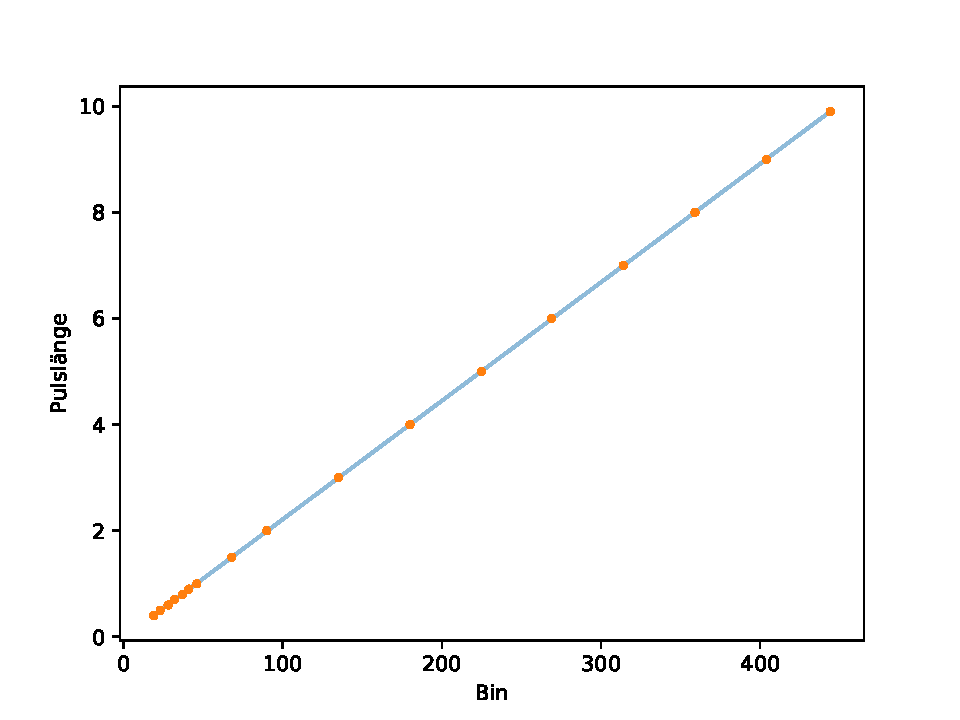
\includegraphics[scale = 1]{./plots/bins.pdf}
    \caption{Die durch den Doppelimpulsgenerator erzeugte Pulsabstand ist gegen die jeweils gefüllten Kanäle des MCA aufgetragen. An die gemessenen Daten wurde eine lineare Ausgleichsgerade genähert. Es ist erkennbar, dass die lineare Ausgleichsgerade die Messdaten gut annähert und daher eine Proportionalität zwischen Pulslänge und Kanal des MCA angenommen werden kann.}
    \label{fig:bins}
\end{figure}
Aus der Annäherung einer linearen Funktion an die Daten ergibt sich der Proportionalitätsfaktor.
\begin{align*}
    \text{Lineare Funktion:}\\
    f(x) &= a \cdot x + b\\
    \text{Parameter:}\\
    a &= \num{0.02234 +- 0.00001}\\
    b &= \SI{ -0.01978 +- 0.00219}{\micro\second}
\end{align*}

\subsection{Bestimmung der Myon Lebenszeit}

\begin{figure}[ht]
    \centering
    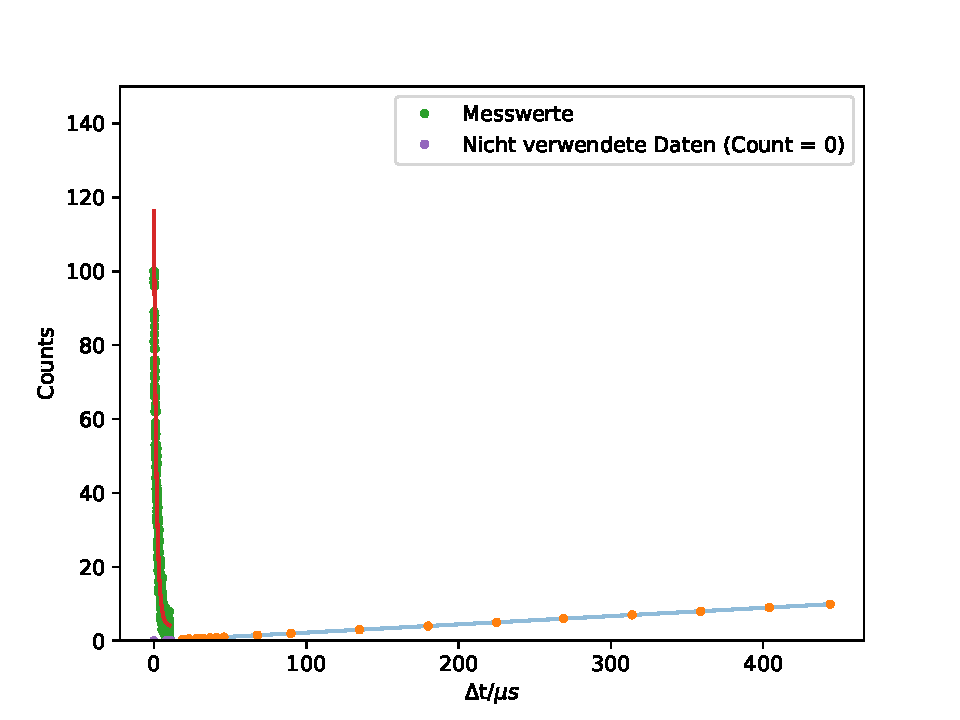
\includegraphics[scale = 1]{./plots/e-fkt.pdf}
    \caption{Die aufgenommenen Counts werden auf die jeweiligen Pulsabstände gebinnt. Kanäle mit einem Count von Null wurden für die anschließende Näherung einer e-Funktion an die Daten entfernt. Die Fehler für die Messwerte ergeben sich genähert durch die Wurzel des jeweiligen Messwertes, da es sich hier um Zählraten handelt. Mit der e-Funktion lassen sich die Daten gut annähern und die Funktion liegt zu jedem Zeitpunkt im Unsicherheitsbereich der Daten.}
    \label{fig:efkt}
\end{figure}

Die Ergebnisse der Messung über 3 Tage sind in Abbildung \ref{fig:efkt} dargestellt.
Die Messdaten zeigen einen exponentiellen Verlauf in den Zeitintervallen zwischen Eintritt des Myons und Zerfall.
Aufgrund des exponentiellen abfallens wird eine e-Funktion an die Daten genähert.
\begin{align*}
    \text{Exponential-Funktion:}\\
    h(t) &= A \cdot \text{exp} \left(-\lambda t\right) + U\\
    \text{Parameter:}\\
    A &= \num{115.2 +- 2.7}\\
    \lambda &= \SI[per-mode=reciprocal]{0.586 +- 0.019}{\per\micro\second}\\
    U &= U_{\text{theo}} = \num{3.105 +- 0.003}\; \frac{\text{Counts}}{\text{Kanal}} \\
\end{align*}
Dabei wurde der Parameter $U$ auf den theoretisch berechneten Untergrund $U_{\text{theo}}$ festgesetzt.

Über das berechnete $\lambda$ lässt sich die Lebensdauer der Myonen bestimmen:
\begin{equation*}
    \tau_{\mu} = \frac{1}{\lambda} = \SI{1.71+-0.05}{\micro\second}
\end{equation*}

\begin{equation*}
    a_{\tau} = \frac{\tau_{\text{theo}} - \tau}{\tau_{\text{theo}}} = \num{0.224 +- 0.026}
\end{equation*}